\documentclass[11pt]{beamer}
\usetheme{CambridgeUS}
\usepackage[utf8]{inputenc}
\usepackage{amsmath}
\usepackage{amsfonts}
\usepackage{amssymb}
\usepackage{graphicx}
\usepackage{pgfpages}
\usepackage{framed}
\usepackage{xcolor}
\usepackage[most]{tcolorbox}
\usepackage{soul}
\usepackage{empheq}

% The replacement character � (often displayed as a black rhombus with a white
% question mark) is a symbol found in the Unicode standard at code point U
% +FFFD in the Specials table. It is used to indicate problems when a system 
% is unable to render a stream of data to a correct symbol.[4] It is usually 
% seen when the data is invalid and does not match any character. For this 
% reason we map explicitly this character to a blanck space.
\DeclareUnicodeCharacter{FFFD}{ }

\newcommand*{\itemimg}[1]{%
  \raisebox{-.3\baselineskip}{%
    \includegraphics[
      height=\baselineskip,
      width=\baselineskip,
      keepaspectratio,
    ]{#1}%
  }%
}

\newtcbox{\mymath}[1][]{%
    nobeforeafter, math upper, tcbox raise base,
    enhanced, colframe=blue!30!black,
    colback=blue!10, boxrule=1pt,
    #1}

\newcommand{\highlight}[1]{%
  \colorbox{yellow!50}{$\displaystyle#1$}}

\author{Giovanni Della Lunga\\{\footnotesize giovanni.dellalunga@unibo.it}}
%\title{2.1 - Data Pre-Processing}
\title{3.1 - Linear and Logistic Regression}
%\title{4.2 - Decision Trees}
%\title{6 - Text Vectorization}
%\title{7 - Classification for Text Analysis}
%\title{8 - Clustering for Text Similarity}
%\title{9 - Information Extraction}
\subtitle{} % (optional)
\setbeamercovered{transparent} 
\institute{Introduction to Machine Learning for Finance} 
\date{Bologna - February, 2022} 

\begin{document}

%\begin{frame}
%\includegraphics[width=\linewidth]{img/halloween-seminar-logo.PNG}
%\end{frame}

\begin{frame}
\titlepage
\end{frame}

\AtBeginSection[]
{
  %\begin{frame}<beamer>
  %\footnotesize	
  %\frametitle{Outline}
  %\begin{multicols}{2}
  %\tableofcontents[currentsection]
  %\end{multicols}	  
  %\normalsize
  %\end{frame}
  \begin{frame}
  \vfill
  \centering
  \begin{beamercolorbox}[sep=8pt,center,shadow=true,rounded=true]{title}  	\usebeamerfont{title}\insertsectionhead\par%
  \end{beamercolorbox}
  \vfill
  \end{frame}
}
\AtBeginSubsection{\frame{\subsectionpage}}

% INSERT HERE
\section{Back to Linear Regression}
%---------------------------------------------------------------------------------------------------
\begin{frame}{Linear Regression}
A linear model makes a prediction by simply computing a weighted
sum of the input features, plus a constant called the \textbf{bias} term (also called the \textbf{intercept}
term):

\begin{equation}
y = b + w_1 X_1 + w_2 X_2 + \dots + w_m X_m + \epsilon
\end{equation}

where:
\begin{itemize}
\item $y$ is the predicted value (the value of the target);
\item $m$ is the number of features;
\item $X_i$ is the $i^{th}$ feature value that are used to predict $y$;
\item $b$ and $w_j$ are the $j^{th}$ model parameters ($b$ being the \textbf{bias} term and $w_i$ the \textbf{weights})
\item $\epsilon$ is the predicton error.
\end{itemize}
\end{frame}
%..................................................................
\begin{frame}{Linear Regression}
\begin{itemize}
\item The parameters $b$ and $w_i$ are chosen to minimize the mean squared error over the training data set. 

\item This means that the task in linear regression is to find values for $b$ and $w_i$ that minimize

\begin{equation}\text{MSE} = 
\frac{1}{n} \sum\limits_{i=1}^n \left(Y - b - w_1 X_{i1} - w_2 X_{i2} - \dots - w_m X_{im} \right)^2
\end{equation}

where $n$ is the size of the training set. 
\end{itemize}
\end{frame}
%..................................................................
\begin{frame}{Linear Regression}
	\begin{center}
	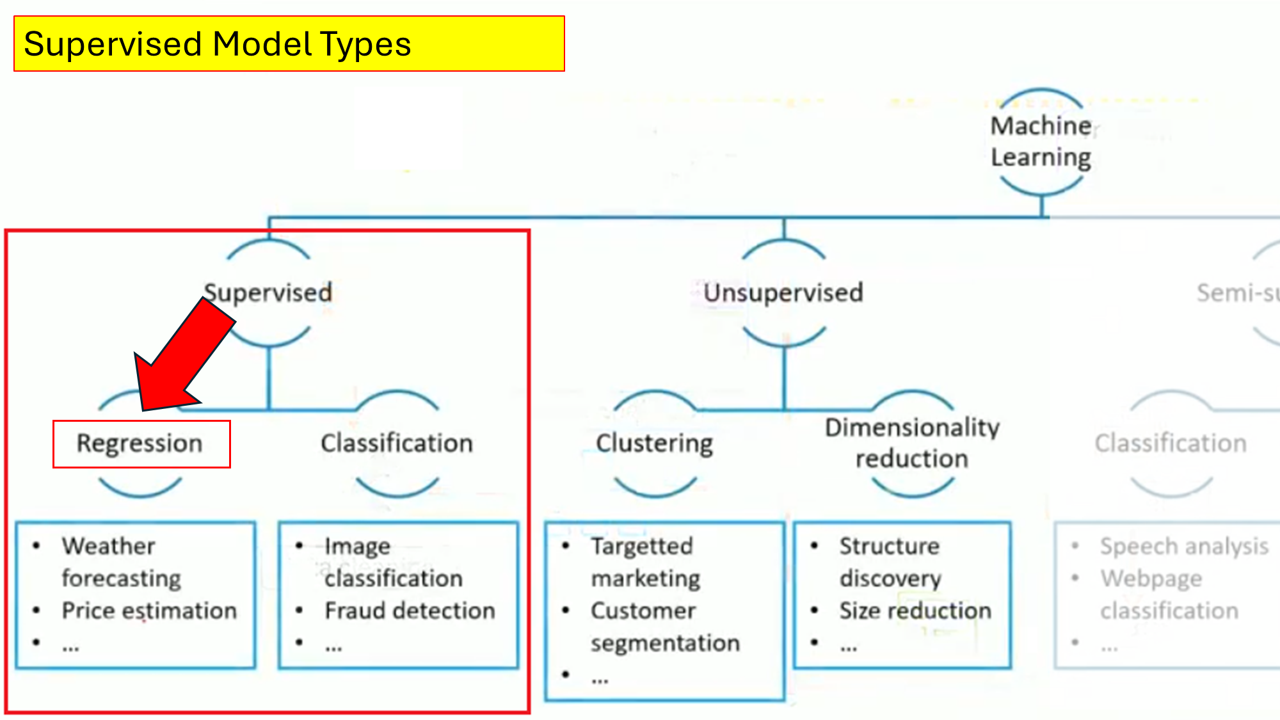
\includegraphics[scale=.35]{../05-pictures/lesson-3-1_pic_0.png}
	\end{center}
\end{frame}
%..................................................................
\begin{frame}{Iowa House Price Case Study}{Linear Regression}
The \textbf{Iowa House Pricing Dataset} from Kaggle is a popular dataset used for regression problems, particularly in the context of machine learning. It contains comprehensive information on houses in Ames, Iowa, and their sale prices, and it was designed to serve as an alternative to the Boston Housing Dataset. Here's a brief overview:
\vspace{.5cm}
\textbf{Dataset Overview}
\begin{itemize}
\item \textbf{Target Variable}: `SalePrice` – the final price of the house in USD.
\item \textbf{Number of Rows (Observations)}: 2,930 (combined training and test datasets).
\item \textbf{Number of Features (Columns)}: 79 explanatory variables plus the target variable.
\end{itemize}

\end{frame}
%..................................................................
\begin{frame}{Iowa House Price Case Study}{Linear Regression}
\begin{center}
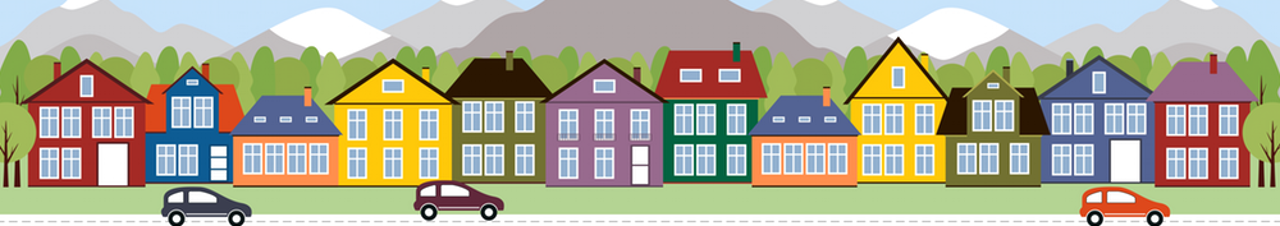
\includegraphics[scale=.3]{../05-pictures/lesson-3-1_pic_1.png} 
\end{center}
	\begin{itemize}
		\item The objective is to predict the prices of house in Iowa from features
		\item 800 observations in training set, 600 in validation set, and 508 in test set
		\item Here the original competition description: \textbf{https://www.kaggle.com/c/house-prices-advanced-regression-techniques}
	\end{itemize}
\end{frame}
%..................................................................
\begin{frame}{Iowa House Price Case Study}{Linear Regression}

\textbf{Types of Features}
\vspace{0.5cm}
The dataset includes a mix of:
\begin{itemize}
\item 1. \textbf{Numerical Features}:\\
   - Continuous (e.g., `LotArea`, `GrLivArea`, `SalePrice`)\\
   - Discrete (e.g., `GarageCars`, `TotRmsAbvGrd`)
\item 2. \textbf{Categorical Features}:\\
   - Nominal (e.g., `Neighborhood`, `HouseStyle`)\\
   - Ordinal (e.g., `ExterQual`, `KitchenQual`)
\item 3. \textbf{Temporal Features}:\\
   - Year-based (e.g., `YearBuilt`, `YrSold`)
\item 4. \textbf{Location Features}:\\
   - Specific location details (e.g., `Neighborhood`, `MSSubClass`).
\end{itemize}
\end{frame}
%..................................................................
\begin{frame}{Iowa House Price Case Study}{Linear Regression}
	Dataset splitting: Training, Validation and Test
	\begin{center}
	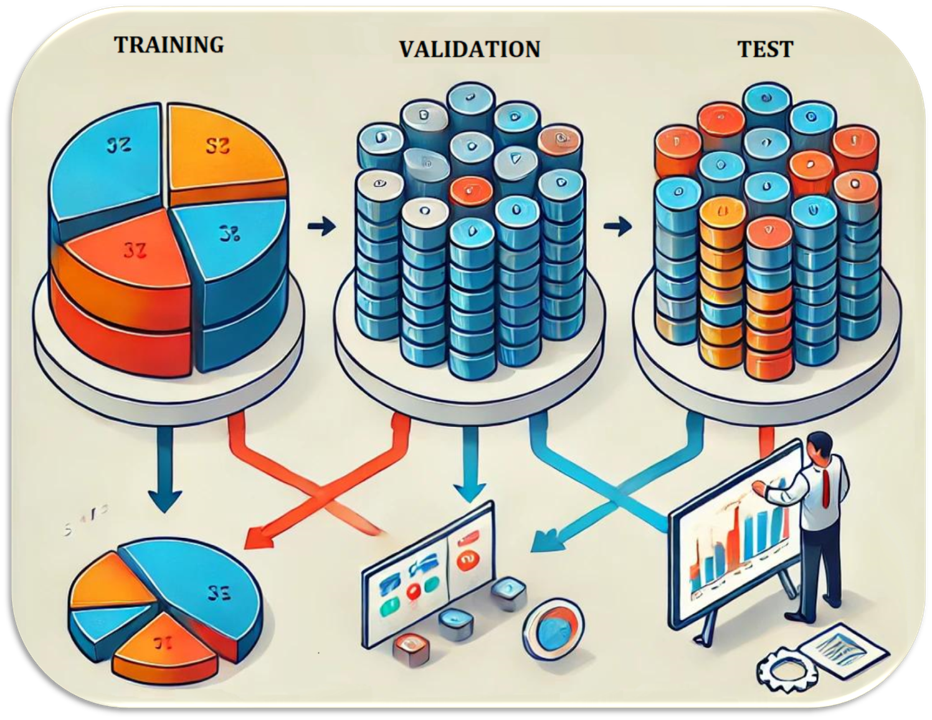
\includegraphics[scale=.3]{../05-pictures/lesson-3-1_pic_2.png}
	\end{center}
\end{frame}
%..................................................................
\begin{frame}{Iowa House Price Results}{Linear Regression}
	\begin{center}
	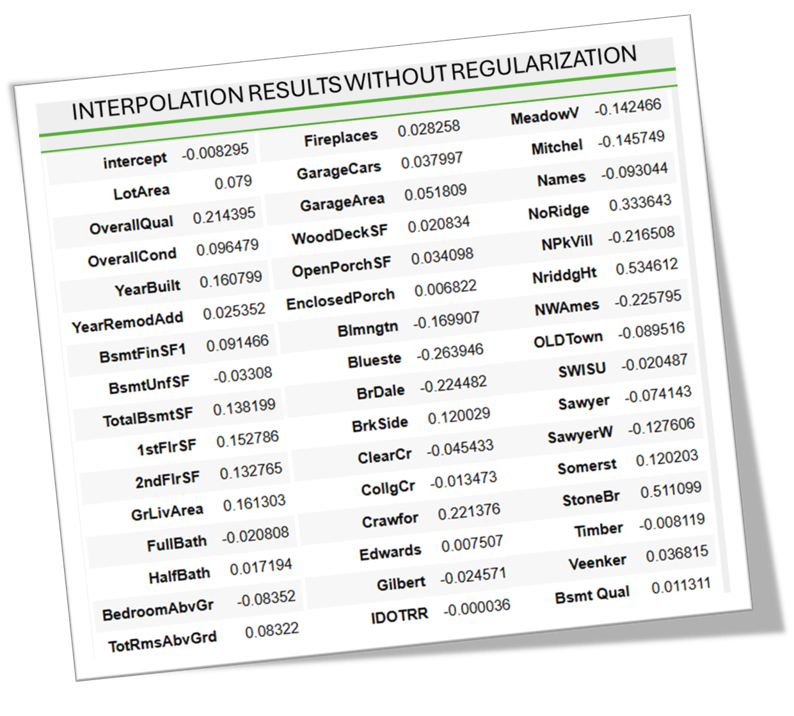
\includegraphics[scale=.4]{../05-pictures/lesson-3-1_pic_3.png}
	\end{center}
\end{frame}
%..................................................................
\begin{frame}{Ridge Regression}{Linear Regression}
We try using Ridge regression with different values of the hyperparameter $\lambda$. The following code shows the effect of this parameter on the prediction error. 
	\begin{center}
	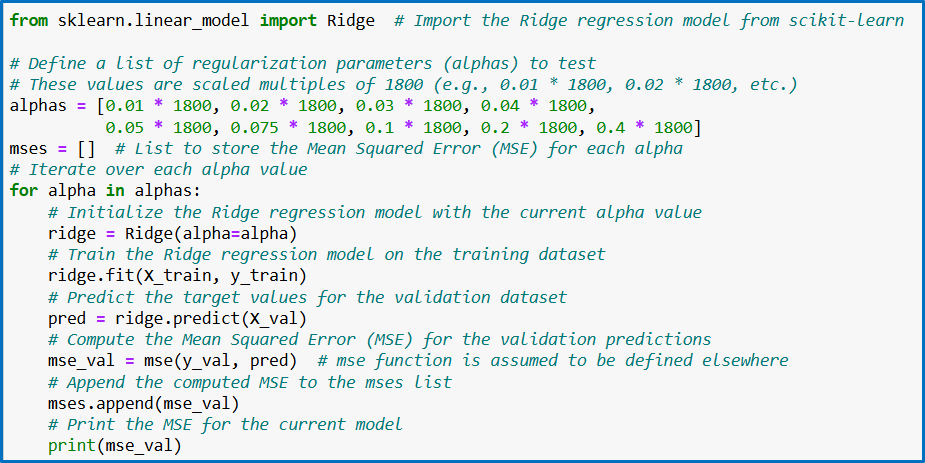
\includegraphics[scale=.45]{../05-pictures/lesson-3-1_pic_4.png}
	\end{center}
\end{frame}
%..................................................................
\begin{frame}{Ridge and Lasso Regression}{Linear Regression}
	\begin{center}
	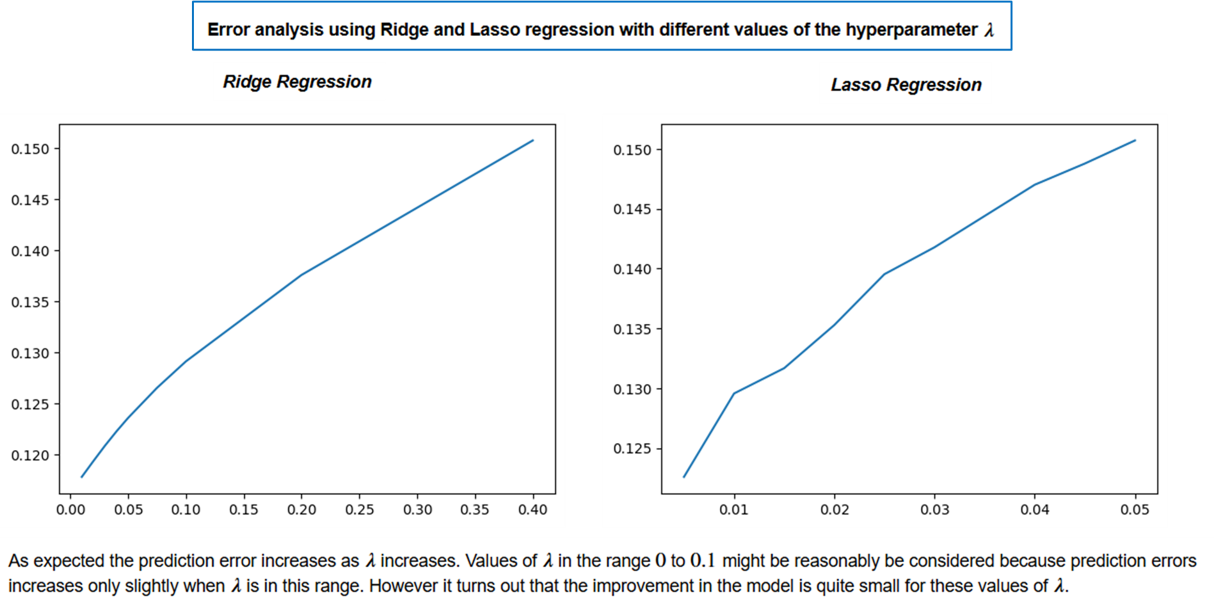
\includegraphics[scale=.38]{../05-pictures/lesson-3-1_pic_5.png}
	\end{center}
\end{frame}
%..................................................................
\begin{frame}{Iowa House Price Results}{Linear Regression}
Non-zero weights for Lasso when $\lambda=0.1$ (overall quality and total living area were most important)
	 
	\begin{center}
	
\includegraphics[scale=.6]{../05-pictures/lesson-3-1_pic_6.png}
	\end{center}
\end{frame}
%..................................................................
\begin{frame}{Summary of Iowa House Price Results}{Linear Regression}
	\begin{itemize}
		\item With no regularization correlation between features leads to some negative weights which we would expect to be positive
		\item Improvements from Ridge is modest
		\item Lasso leads to a much bigger improvement in this case
		\item Elastic net similar to Lasso in this case
		\item Mean squared error for test set for Lasso with $\lambda=0.1$ is 14.7\\% so that 85.3\\% of variance is explained
	\end{itemize}
\end{frame}

%..................................................................
\section{Logistic Regression}
%..................................................................
\begin{frame}{Logistic Regression}
	\begin{center}
	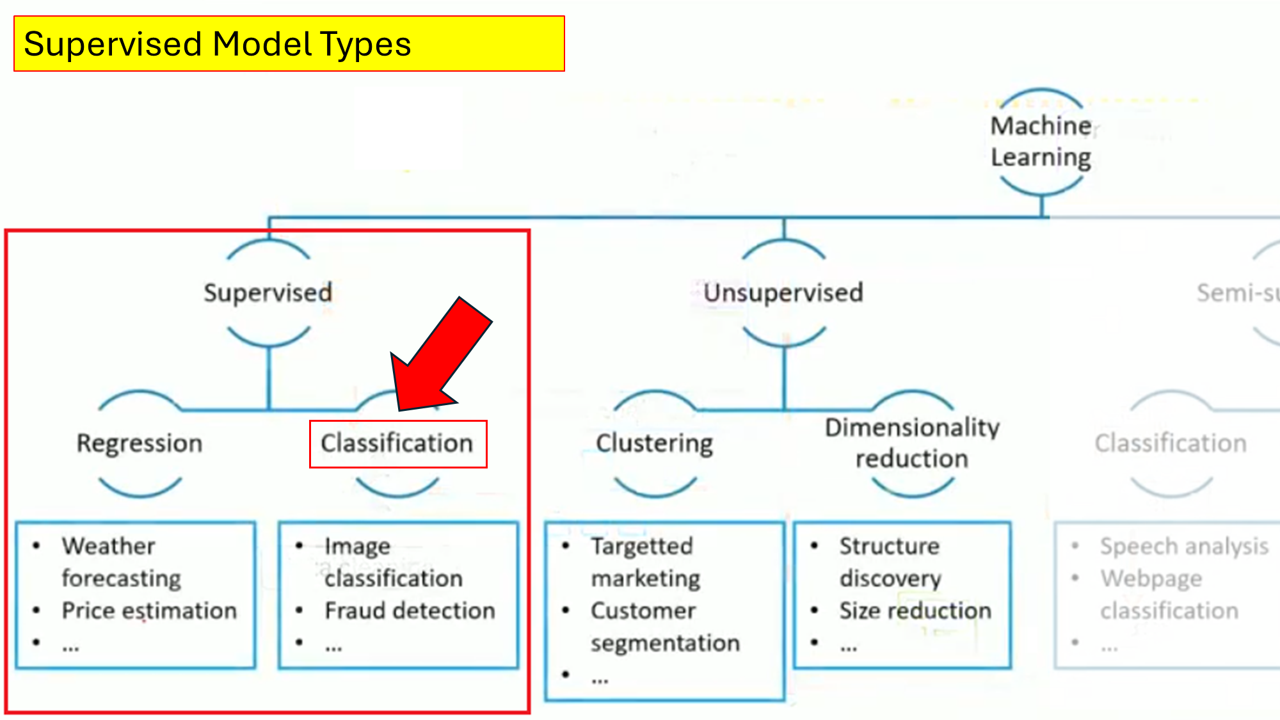
\includegraphics[scale=.35]{../05-pictures/lesson-3-1_pic_7.png}
	\end{center}
\end{frame}
%---------------------------------------------------------------------------------------------------
\begin{frame}{Logistic Regression}
	\begin{itemize}
		\item The objective is to classify observations into a \textbf{positive outcome} and \textbf{negative outcome} using data on features
		\item Probability of a positive outcome is assumed to be a sigmoid function: \begin{equation} Q = \frac{1}{1+e^{-Y}}\end{equation}
		\item    where $Y$ is related linearly to the values of the features: \begin{equation}Y=a+b_1X_1 + b_2X_2 + \dots + b_mX_m\end{equation}
	\end{itemize}
\end{frame}
%..................................................................
\begin{frame}{Logistic Regression}
	\begin{center}
	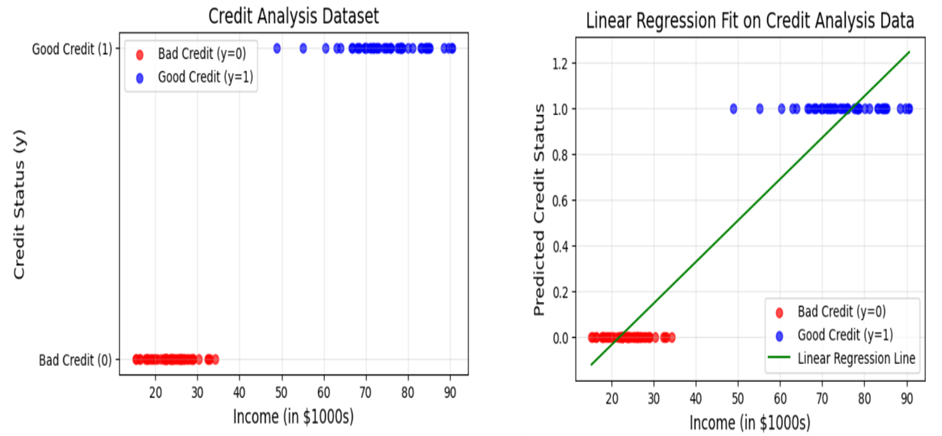
\includegraphics[scale=.45]{../05-pictures/lesson-3-1_pic_8.png}
	\end{center}
\end{frame}
%..................................................................
\begin{frame}{The Sigmoid Function}
	\begin{center}
	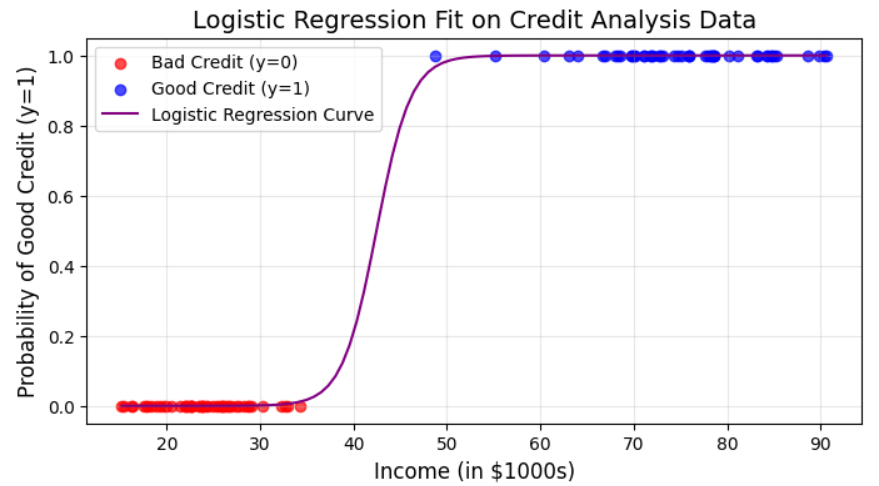
\includegraphics[scale=.45]{../05-pictures/lesson-3-1_pic_9.png}
	\end{center}
\end{frame}
%..................................................................
\begin{frame}{Maximum Likelihood Estimation}
	\begin{itemize}
		\item We use the training set to maximize
		\item \begin{equation}L=\sum\limits_\text{POS OUT} \, \ln(Q) + \sum\limits_\text{NEG OUT} \, \ln(1-Q) \end{equation}
		\item This cannot be maximized analytically but we can use a gradient ascent algorithm
	\end{itemize}
\end{frame}
%..................................................................
\begin{frame}{Confusion Matrix}
	\begin{center}
	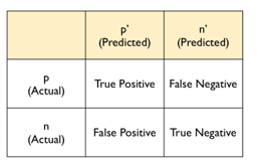
\includegraphics[scale=1]{../05-pictures/lesson-3-1_pic_10.png}
	\end{center}
\end{frame}
%..................................................................
\begin{frame}{Lending Club Case Study}
	\begin{itemize}
		\item Data consists of loans made and whether they proved to be good or defaulted. (A restriction is that you do not have data for loans that were never made.)
		\item We use only four features
		\item Home ownership (rent vs. own)
		\item Income
		\item Debt to income
		\item Credit score
		\item Training set has 8,695 observations (7,196 good loans and 1,499 defaulting loans). Test set has 5,196 observations (4,858 good loans and 1,058 defaulting loans)
	\end{itemize}
\end{frame}
%..................................................................
\begin{frame}{The Data}
	\begin{center}
	
\includegraphics[scale=0.5]{../05-pictures/lesson-3-1_pic_11.png}
	\end{center}
\end{frame}
%..................................................................
\begin{frame}{Results for Lending Club Training Set}
	\begin{itemize}
		\item $X_1$= Home Ownership
		\item $X_2$= Income
		\item $X_3$= Debt to income ratio
		\item $X_4$ = Credit score
		\item $$Y=-6.5645+0.1395\cdot X_1+0.0041\cdot X_2-0.0011\cdot X_3+0.0113\cdot X_4$$
	\end{itemize}
\end{frame}
%..................................................................
\begin{frame}{Decision Criterion}
	\begin{itemize}
		\item The data set is imbalanced with more good loans than defaulting loans
		\item There are procedures for creating a balanced data set
		\item With a balanced data set we could classify an observation as positive if $Q>0.5$ and negative otherwise
		\item However this does not consider the cost of misclassifying a bad loan and the lost profit from misclassifying a good loan
		\item A better approach is to investigate different thresholds, $Z$
		\item If $Q>Z$ we accept a loan
		\item If $Q\le Z$ we reject the loan
	\end{itemize}
\end{frame}
%..................................................................
\begin{frame}{Test Results}
	See Hull, Tables 3.10, 3.11, and 3.12 
	\begin{center}
	
\includegraphics[scale=1]{../05-pictures/lesson-3-1_pic_12.png}
	\end{center}
\end{frame}
%..................................................................
\begin{frame}{The Confusion matrix and common ratios}
	\begin{center}
	
\includegraphics[scale=0.5]{../05-pictures/lesson-3-1_pic_13.png}
	\end{center}
\end{frame}
%..................................................................
\begin{frame}{Test Set Ratios for different Z values}
	 
	\begin{center}
	
\includegraphics[scale=0.5]{../05-pictures/lesson-3-1_pic_14.png}
	\end{center}
\end{frame}
%..................................................................
\begin{frame}{As we change the Z criterion we get an ROC}
	 
	\begin{center}
	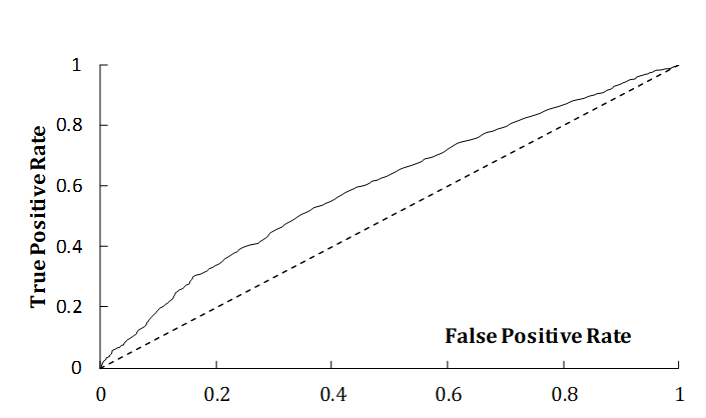
\includegraphics[scale=0.5]{../05-pictures/lesson-3-1_pic_15.png}
	\end{center}
\end{frame}
%..................................................................
\begin{frame}{Area Under Curve (AUC)}
	\begin{itemize}
		\item The area under the curve is a popular way of summarizing the predictive ability of a model to estimate a binary variable
		\item When $AUC =1$ the model is perfect. 
		\item When $AUC =0.5$ the model has no predictive ability
		\item When $AUC<0.5$ the model is worse than random
		\item In this case $AUC = 0.6020$
	\end{itemize}
\end{frame}
%..................................................................
\begin{frame}{Choosing Z}
	\begin{itemize}
		\item The value of $Z$ can be based on 
		\item The expected profit from a loan that is good, $P$
		\item The expected loss from a loan that defaults, $L$
		\item We need to maximize: $P \times \text{TP}-L \times \text{FP}$
	\end{itemize}
\end{frame}
%..................................................................
%=====================================================================

\end{document}

%..................................................................
\begin{frame}{Linear Regression}

\end{frame}
%..................................................................
\begin{frame}{Linear Regression}

\end{frame}
%..................................................................
\begin{frame}{Linear Regression}

\end{frame}
%..................................................................
\begin{frame}{Linear Regression}

\end{frame}
%..................................................................
\begin{frame}{Linear Regression}

\end{frame}
%..................................................................
\begin{frame}{Linear Regression}

\end{frame}
